\section{Resting atmosphere}
\label{sec:resting}

This two-dimensional test simulates a stably stratified atmosphere in hydrostatic balance.  Since there are no net forces, the analytical solution should remain at rest.  The test specification follows that from \textcite{klemp2011}.  \TODO{again, what is this designed to test?  Klemp says the horiz pressure gradient.  Good says the inversion layer introduces nonlinearity to tax the model even more}

\subsection{Specification}
Following \textcite{weller-shahrokhi2014}, the domain is \SI{20}{\kilo\meter} wide and \SI{20}{\kilo\meter} high, which is narrower than \textcite{klemp2011} in order to reduce simulation time.  The wave-shaped mountain profile is taken from \textcite{schaer2002} where the surface height $h$ is given by
\begin{align}
\surface(x) = \surface_0 \exp \left( - \left( \frac{x}{a} \right)^2 \right) \cos^2 \left( \frac{\pi x}{\lambda} \right)
\end{align}
where $a = \SI{5}{\kilo\meter}$ is the mountain half-width, $h_0 = \SI{1}{\kilo\meter}$ is the maximum mountain height and $\lambda = \SI{4}{\kilo\meter}$ is the wavelength.  For the SLEVE grid, the large-scale component $\surface_1$, described in section~\ref{sec:theory:sleve}, is specified as
\begin{align}
\surface_1(x) = \frac{1}{2} \surface_0 \exp \left( - \left( \frac{x}{a} \right)^2 \right)
\end{align}
and, following \cite{leuenberger2010}, $s_1 = \SI{4}{\kilo\meter}$ is the large scale height, $s_2 = \SI{1}{\kilo\meter}$ is the small scale height, and the optimal exponent value of $n = 1.35$ is used.  Results are compared with the numerical solution with no orography.

The initial thermodynamic conditions have a surface temperature of $\theta_0 = \SI{288}{\kelvin}$ and constant stability with Brunt-V\"ais\"al\"a frequency $N = \SI{0.01}{\per\second}$ everywhere, except for a more stable layer of $N = \SI{0.02}{\per\second}$ between $\SI{2}{\kilo\meter} \leq z \leq \SI{3}{\kilo\meter}$.

\subsection{Diagnostics}
Two metrics were used to measure the model error.  First, maximum vertical velocity is measured at each timestep.  An analytic solution has no vertical velocity $w$ since the atmosphere is at rest.  However, numerical error in calculating the horizontal pressure gradient give rise to spurious vertical velocities which become more severe over steep terrain \autocite{klemp2011}.

Second, normalised energy change $\Delta E$ is measured for each timestep by comparing with the energy in the initial conditions, that is
\begin{align}
	\Delta E(t) &= \frac{E(t) - E(t = \SI{0}{\second})}{E(t = \SI{0}{\second})}
%
	\intertext{where energy is kinetic $E_K$, potential $E_P$, or internal $E_I$, given by \TODOsidenote{check these with Hilary}}
%
	E_K &= \frac{0.25 \sum_{surface} \frac{UV}{\rho}}{\sum V} / \sum_{cells} V \\
	E_P &= - \int_V \rho \vect{g} \cdot \vect{x_c} \\
	E_I &= \int_V \rho \theta \Pi c_v
\end{align}
An analytic solution would conserve energy such that $\Delta E(t) = 0\;\forall\;t$.  \TODO{why would we expect our model to lose energy?}

\subsection{Discretisation}
The simulation uses the discretisation of the fully-compressible Euler equations described in section~\ref{sec:method:discretisation}.  The domain is discretised on a grid having $40 \times 40$ cells such that $\Delta x = \Delta z = \SI{0.5}{\kilo\meter}$.  All boundary conditions are no slip.  The simulation is integrated forward by 5 hours with a timestep $\Delta t = \SI{100}{\second}$.  Unlike \textcite{klemp2011}, there is no eddy diffusion in our equation set.


\subsection{Results}
\begin{figure}
	\captionsetup[subfigure]{position=b}
	\centering
	\subcaptionbox{Model results}[0.58\textwidth]{\input{resting-w-plot}}
	\hfill
	\subcaptionbox{Results from \textcite{klemp2011}}[0.4\textwidth]{\vspace{0.27in}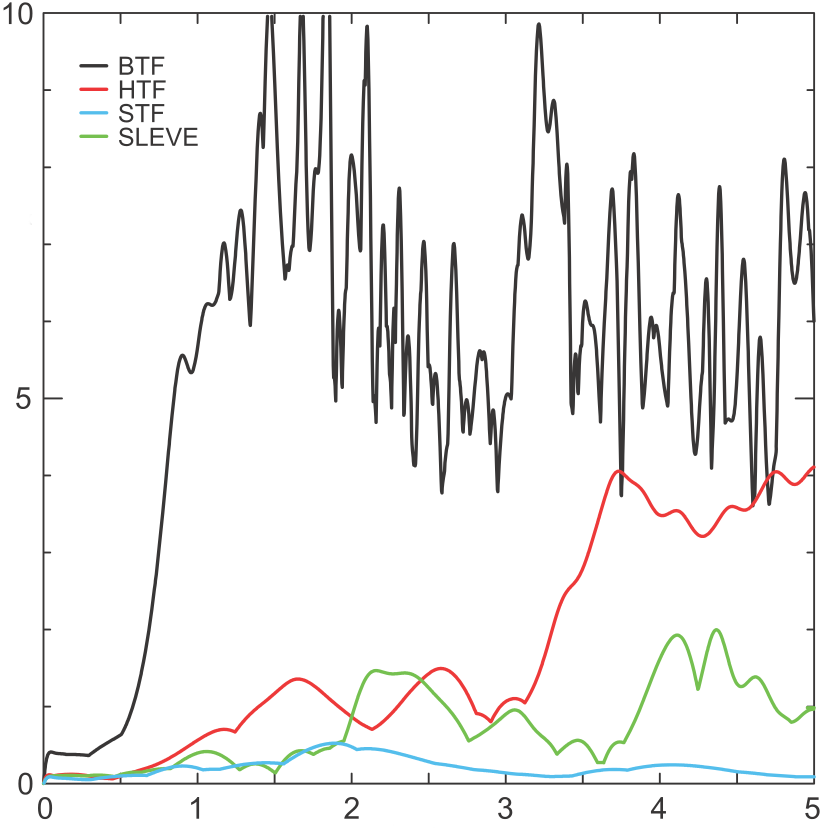
\includegraphics[height=2in]{img/klemp-w.png}}
	\caption{Maximum spurious vertical velocity $w$ in the resting atmosphere test compared with results from \textcite{klemp2011}.  Note that vertical scales differ.}
	\label{fig:resting:w}
\end{figure}

Test results for BTF, optimised SLEVE, and SnapCol grids are compared with results on a regular grid with no orography.  On the BTF grid, spurious vertical velocity $w$ reaches $\sim \SI{35}{\centi\meter\per\second}$, which is significantly less than the velocities of $\sim \SI{10}{\meter\per\second}$ found by \textcite{klemp2011} (see figure~\ref{fig:resting:w}, note different vertical scales).  A computational oscillation develops after 4 hours, the cause of which is not yet known.  The optimised SLEVE grid does not significantly reduce $w$ compared to BTF; in fact, an increase is seen at some points during the simulation.  Since the model and its initialisation are the same, results on the BTF and optimised SLEVE grids are also in agreement with \textcite{weller-shahrokhi2014}.

The SnapCol grid results in a significantly smaller maximum vertical velocity of less than \SI{1}{\milli\meter\per\second}.  The smallest error of $\sim \SI{1e-10}{\meter\per\second}$ is found on the regular grid.  This error may be due to loss of precision when OpenFOAM loads the initial conditions, which are in discrete hydrostatic balance, but the source of the error is not certain.  Using a timestep of \SI{1.01}{\second}, \textcite{good2013} found the maximum vertical velocity in their cut cell model was \SI{1e-12}{\meter\per\second}, which is better than any result from our experiments.

\begin{figure}
	\captionsetup[subfigure]{position=b}
	\centering
	\subcaptionbox{Total normalised energy changes}[0.48\textwidth]{\input{resting-energy-total-plot}}
	\hfill
	\subcaptionbox{BTF}[0.48\textwidth]{\input{resting-energy-btf-plot}}
	\\
	\subcaptionbox{Optimised SLEVE}[0.48\textwidth]{\input{resting-energy-sleve-plot}}
	\hfill
	\subcaptionbox{SnapCol (note different vertical scale from other plots)}[0.48\textwidth]{\input{resting-energy-snapCol-plot}}
	\caption{\TODO{Normalised energy changes}}
	\label{fig:resting:energy}
\end{figure}

\TODO{compare total energy changes between grids}

\TODO{discuss individual energy changes (KE/PE/IE) between grids}

\TODO{if I want to compare to Zaengl (and also Good), I would need to try the same experiment with 4km high mountain, too}

\TODO{Although I did experiment with Hop vs dp/dx, I'm not sure how valuable it is to discuss here.  I don't currently have results of SnapCol Hop vs dp/dx.}

\TODO{I could compare theta field (as done by Klemp)}


\hrule

\begin{figure}
BTF H
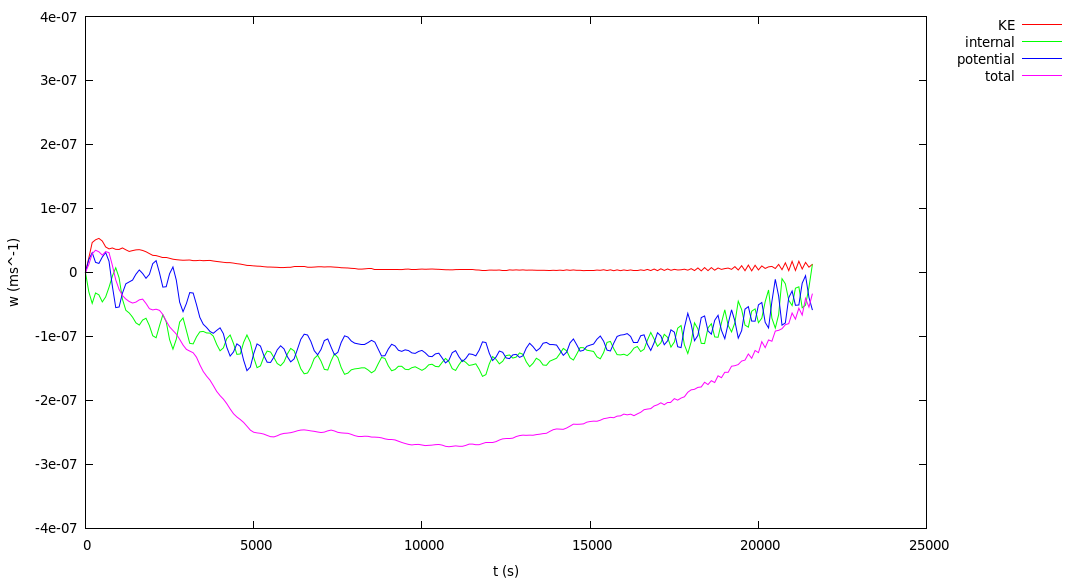
\includegraphics[width=\textwidth]{interim-results/restingBtfHEnergy.png}
SLEVE
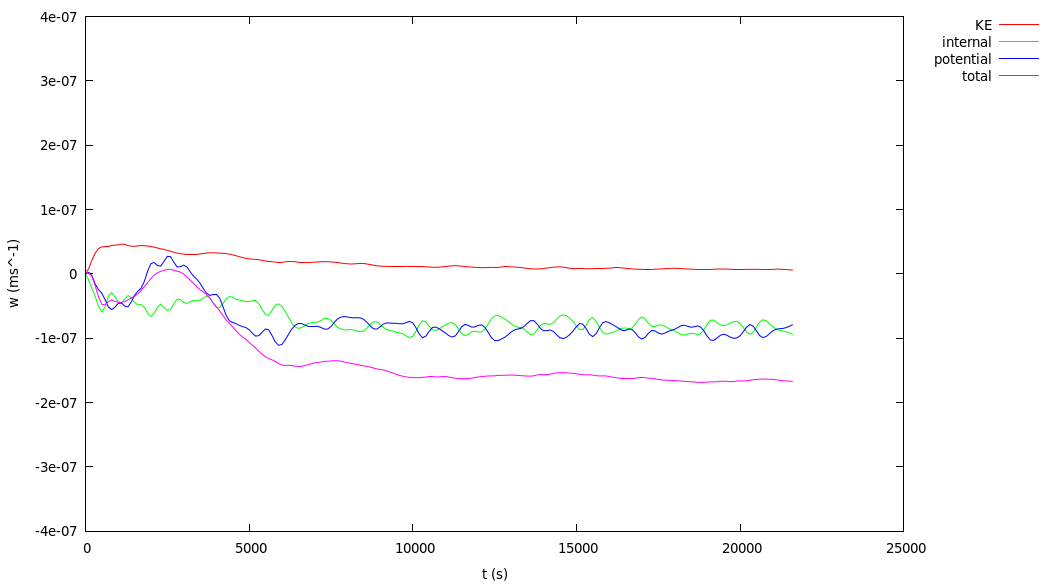
\includegraphics[width=\textwidth]{interim-results/restingSleveEnergy.png}
\caption{Energy changes (TF)}
\label{fig:rest:energy-tf}
\end{figure}

\begin{figure}
SnapCol
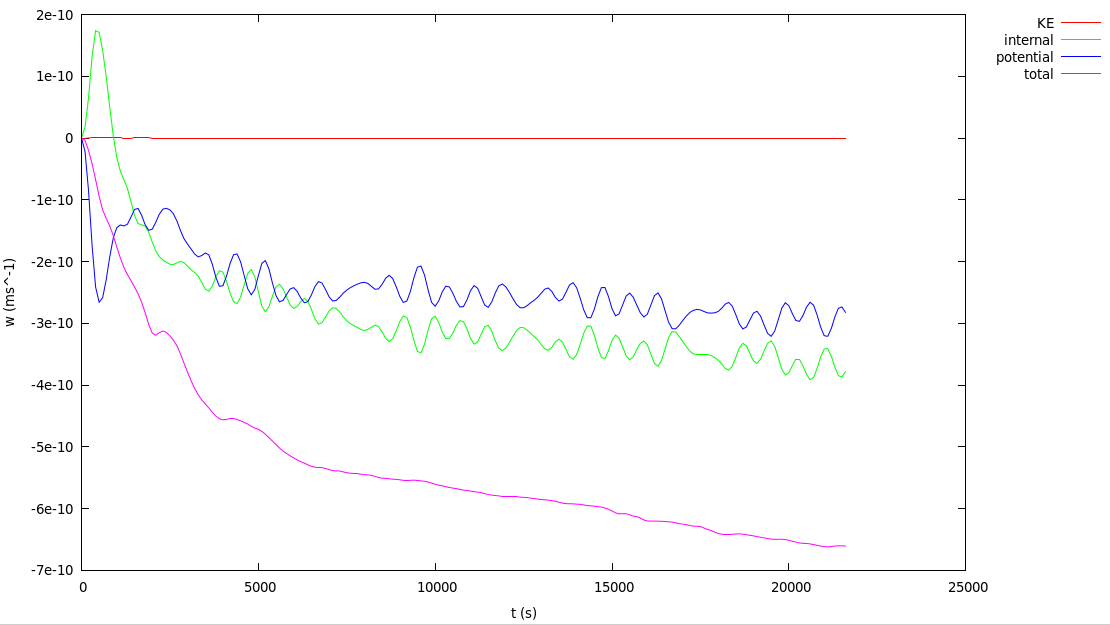
\includegraphics[width=\textwidth]{interim-results/restingSnapColEnergy.png}
\caption{Energy changes (cut-cell style)}
\label{fig:rest:energy-cut-cell}
\end{figure}
